\chapter{Conclusion}
\label{chap:conclusion}

\chapterquote{Overview first, zoom and filter, then details-on-demand}
{Ben Schneiderman, 1996}

\newpage
{\footnotesize \hypersetup{linkcolor=black}
\minitoc}

\section{Future Work}
During the journey of the thesis, there were many avenues that the thesis could have followed. As such, we dedicate this section to discussing some of these ideas, as well as potential directions a subsequent candidate could follow during their PhD.

With regards to our literature review, We feel we have opened the doors to a range of potential survey papers under the SoS, or meta-survey branch. During the process of the thesis, other related surveys have been published \cite{alharbi2017molecular, alharbi2018sos, rees2019survey}. However, other avenues could be presented such as a Survey of Surveys for Geospatial, Scientific or Computer Graphics.

There are many avenues for future work for the merging algorithm presented in the thesis. Although we use real unit-areas, we would like to test with a broader range of choropleth data. The algorithm still has performance optimizations which could accelerate the speed even further, such as schematization \cite{barkowsky2000schematizing} which could be used to enable better optimization with the drawback of topological continuity being reduced. Other existing formats such as TopoJSON \cite{bostock2018topojson} look at reducing geometry redundancy and could be an excellent subsequent format for the procedure. The current termination method revolves around the idea of one area per contiguous region. Updates in the procedure could allow for more user control when it comes to stopping the merge procedure such as for categorical data where the most abstraction is introduced. Alternatively to this, a bi-variate color map could be implemented to display more accurate concordance of underlying values.  The algorithm potentially can apply to any data-sets with geometric boundaries and is open to new data structures. 

There are some limitations to the study we review in Chapter \ref{chap:userStudy}. We found boundary design to be a more significant factor for small area sizes than anticipated. In the pilot study, we found that users had a much better accuracy overall, and comments were made about the area's color changing. This was actually due to the boundary's framing of the pixel, enhancing the perception of color based on the surrounding black contour. We try to control this as carefully as possible, however, this could be examined further in a follow-up study. We use real-world maps and areas. This means we do not control the aspect ratio of the areas, which may lead to more error in some situations such as narrow areas. This is an aspect that can be explored in an alternative study. T1 and T2 could point to a large amount of future research. For example, since we hold data about the location of the presented area and the color seeding, we could look back at what could have influenced the color perception and decision for the area.

For our multivariate implementation in Chapter \ref{chap:MultivariateMaps}. At the moment, we use the raw derived centroid as a placement strategy. Although this removes a lot of density and occlusion, there is still some wasted space. We believe that by adding some overlap removal, we could use space more efficiently, while still avoiding any decoupling problems. Although we present some case studies, the algorithm could be more carefully compared to other glyph placement strategies with a user-study evaluation. We think the use of transitions is a great tool for understanding variation, but it is not always necessary. We feel that there are many avenues for exploring at multiple levels of detail. For example, directly zooming to a glyphs unit area extents may not need to represent zooming, to speed up exploration.

Now that we can improve performance on a second pass-through by saving build instructions to reduce the calculation of neighbor and boundaries, the next step would be to pipe multiple areas to be merged. This would allow the user to constrain area representation to the desired representation further. For example, if we look at the UK, OA's would only merge within their LSOA, and LSOA's would only merge within their MSOA's.

At the Vis 2015 conference, Ribarksy states "When you add dimensions to a problem, all of a sudden it becomes unsolved" \cite{ribarsky2015solved}. Although we extend our technique to take advantage of multivariate data. There are still opportunities to increase the dimensionality by asking for both statistical and temporal data at once.

We worked with 2D coordinate-spaces. A 3D coordinate space would be an exciting direction to take the algorithm and could open new applications for the process. This would not be a trivial conversion, however. The first thing we would need to consider would be complexity. As of the publication of the thesis. The algorithm relies heavily on vertex checking to make sure that we do not miss vital boundary points by increasing the dimensions by $n$, we scale the boundary search by $n$. The benefit is that even with this, modifying our saved instructions files to represent 3D data should enable us to run the algorithm at reasonable times in second-runthroughs. In terms of our boundary identification, we have to review non-manifold geometry. Marcheix and Gueorguieva define non-manifold geometries as \textit{"a topological space where every point has a neighborhood topologically equivalent to $D^n(x,r) = \{ y \in R^n : \left \| x-y \right \| < r \}$", considered dimensionally unhomogeneous objects} \cite{marcheix1995topological}. We could either allow non-manifold geometries altogether, allow specific instances (2-vertex boundaries only, for example), or completely ignore non-manifold geometries from being considered. See Figure \ref{fig:manifold} for examples of non-manifold geometries.
\begin{figure}[t]
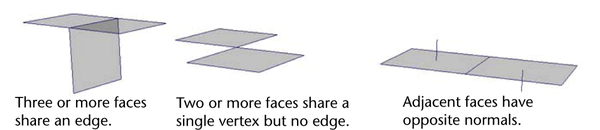
\includegraphics[width=0.7\textwidth]{images/ch7/nonmanifold}
\caption{Examples of non-manifold geometries. Courtesy of Autodesk \cite{autodesk_2019}.} \label{fig:manifold}
\end{figure}
Moving on from here, identifying common vertices would also need to be modified. We rely on order vertex lists however this is a more complex situation when identifying 3D points. it may be smarted to incorporate search trees to identify when a shared boundary is found. One of the new challenges that would need to be considered is how to effectively use an amalgamation technique who holds the detail of edge boundaries over existing techniques. With 3D models, vertexes aren't as important to a surface as they are in a 2D environment. It would be interesting to see how users perceive non-shared surfaces against less strict aggregation methods such as divide and conquer1 \cite{boissonnat1998algorithmic}. We would love to see how people can effectively use this algorithm to highlight strict edge unification with 3D data. 3D projection of 2D coordinate spaces would also be an interesting way forward with this work.

In order to move full circle (refer to Chapter \ref{chap:SoS}), we must consider scalability as our future work. Although throughout the thesis, we made large leaps in both the scale and performance, we still met some challenges in the area. During our initial testing of the algorithm, we attempted to run the algorithm on some large datasets, including the output areas of Wales and England. This dataset held over 180,000 polygons with high complexity vertex lists. Although our algorithm did not fail, the performance time became such an issue (days) that we had to terminate before we could see any result. If there was more time, I believe that search for ways to optimize the algorithm in order to make this dataset achievable would be a good next step. Some options for this would be more focus on GPU implementation, multi-threaded processing, and a way to hold contiguous structures separately from the build hierarchy to avoid unnecessary recalculation.

\section{Conclusion} \label{sec:conclusion}
We conclude all of the discussion within the thesis. 

In Chapter \ref{chap:intro}, we give an introduction to the topic, and where it fits into the overarching field of data visualization.

In Chapter \ref{chap:SoS}, the SoS contributes a step forward in literature surveys. We present a novel classification of survey papers that enables the reader to find recently published literature among a wide variety of topics. The classification also enables users to easily spot areas of open-research for survey publication, as well as an understanding of broad open research topics in the field of information visualization. The literature review provides a basic systematization of classification tables among the existing survey literature. It provides a valuable starting point for both newcomers and experienced researchers in visualization. We also believe it provides a valuable resource to readers outside of the information visualization and visual analytics communities. 

In Chapter \ref{chap:dcm}, we introduce a novel method of smooth and continuous zooming by exploiting a hierarchical data structure to merge areas based on their sizes and shared boundary. The shared boundary is found by first comparing the vertex list of two neighboring areas and finding the longest vertex chain between common vertices. We then render only the perceivable areas or area clusters based on the current zoom level and screen space. This method of rendering improves perceptibility whilst still providing an understanding of the underlying data without distorting the map. This enables the user to zoom without any distortion to the geometry and enables clear perceivable choropleth data for the user. 

In Chapter \ref{chap:userStudy}, we conduct a preliminary study to evaluate perceptual evaluation of performance error, performance time, and preference of area's relative to size in choropleth maps. We hypothesize that the smaller the size of a unit area, the higher the error rate of perceiving the correct underlying color category; the smaller the unit area, the more time required to perceive its color; and the user will prefer choropleth maps with a larger minimum size over those with smaller sizes. Particularly, users will prefer a trade-off between area resolution in favor of legibility. For these three statements, we support the first two using Pearson's r to show a relationship between the variables, with strong observations for the third that give an initial understanding of how users' perceive the relationship between area size and data on a choropleth map. We recommend at least 10 pixels displayed for each area to be accurately interpreted.

In Chapter \ref{chap:MultivariateMaps}, we present a glyph placement algorithm supporting multivariate geospatial visualization at different levels of detail.  We discuss how we create scale aware map, and apply the process to glyph placement. We also discuss the different glyph options and filters we have designed to support the exploration of multivariate data. Finally, we review the algorithm by examining the separate use cases and compare against a pre-existing glyph placement strategy. We also discuss the concept of data abstraction to create low fidelity visualization. We look at perception as well as the idea of hiding or anonymizing data, and some considerations that need to be taken into account when creating them.

In Chapter \ref{chap:softdev}, we discuss some of the more interesting challenges that were overcome within software development, including debug visualization, intersection testing, and the complexities of identifying boundaries.

Finally in Chapter \ref{chap:conclusion}, we conclude our thesis with some avenues for future work and conclusions. In Our Appendix \ref{chap:howTo}, we also present an educational piece on how to write a visualization survey paper.